\label{sec:ndsResults}
%\subsection{Проблемы проектирования}

С помощью сформированной расчетной МКЭ-модели были проведены прочностные исследования напряженно-деформированного состояния(НДС) модели гипотетического БПЛА в рамках проектировочного исследования по определению рациональных параметров конструкции центроплана. 
Из-за существенного влияния жесткостных параметров конструкции планера БПЛА на прочностные параметры конструкции центроплана это проектировочное исследование включало всю первичную конструкцию БПЛА. На основе начальных данных, полученных аналитическим способом, была проведена оптимизация толщин панелей и стенок отсеков для нахождения минимальной по весу конструкции, удовлетворяющей требованиям прочности. Условия по устойчивости анализировались в автоматическом режиме лишь для подкрепленных панелей центроплана и кессона крыла.

Для модели, полученной в результате определения рациональных параметров, можно выделить следующие особенности НДС:

\begin{enumerate}
\item Усилия в обшивке фюзеляжа оказались относительно малы за исключением обшивки центроплана. Поэтому большая часть обшивки имела минимальную толщину, определяемую геометрическими и технологическими ограничениями.
\item Наибольшие усилия наблюдались в центроплане и в корне крыла. Так, в корне крыла наблюдались следующие величины усилий: $Q = 13,7~\text{тс}$, $M_\text{изг} = 80~\text{тс}\cdot\m$. 
\item Значительные усилия наблюдались в стенках отсека двигателя в местах крепления двигателя (дополнительный анализ этой особенности произведен далее в данном разделе). 
\item Влияние кручения крыла мало относительно изгиба крыла. На Рис.\ref{fig:WingDeformation3},\ref{fig:WingRotating} показаны эпюры прогибов лонжеронов при изгибе и кручении крыла.
\end{enumerate}  

Общая картина НДС расчетной модели БПЛА представлена на Рис.\ref{fig:patranRearDeformed}--\ref{fig:patranTopIsoWithoutSk}


\begin{figure}[H]
\centering

\captionsetup{justification=centering}
\def\svgwidth{0.9\textwidth}
\input{figures/WingDeformation3.pdf_tex}
\caption{Эпюры прогибов лонжеронов, полученные в результате расчетов МКЭ- и балочной моделей}
\label{fig:WingDeformation3}
\end{figure}

\begin{figure}[H]
\centering
\def\svgwidth{0.9\textwidth}
\input{figures/WingRotating.pdf_tex}
\caption{Кручение крыла. Разность прогибов лонжеронов}
\label{fig:WingRotating}
\end{figure}


\begin{figure}[H]
\centering
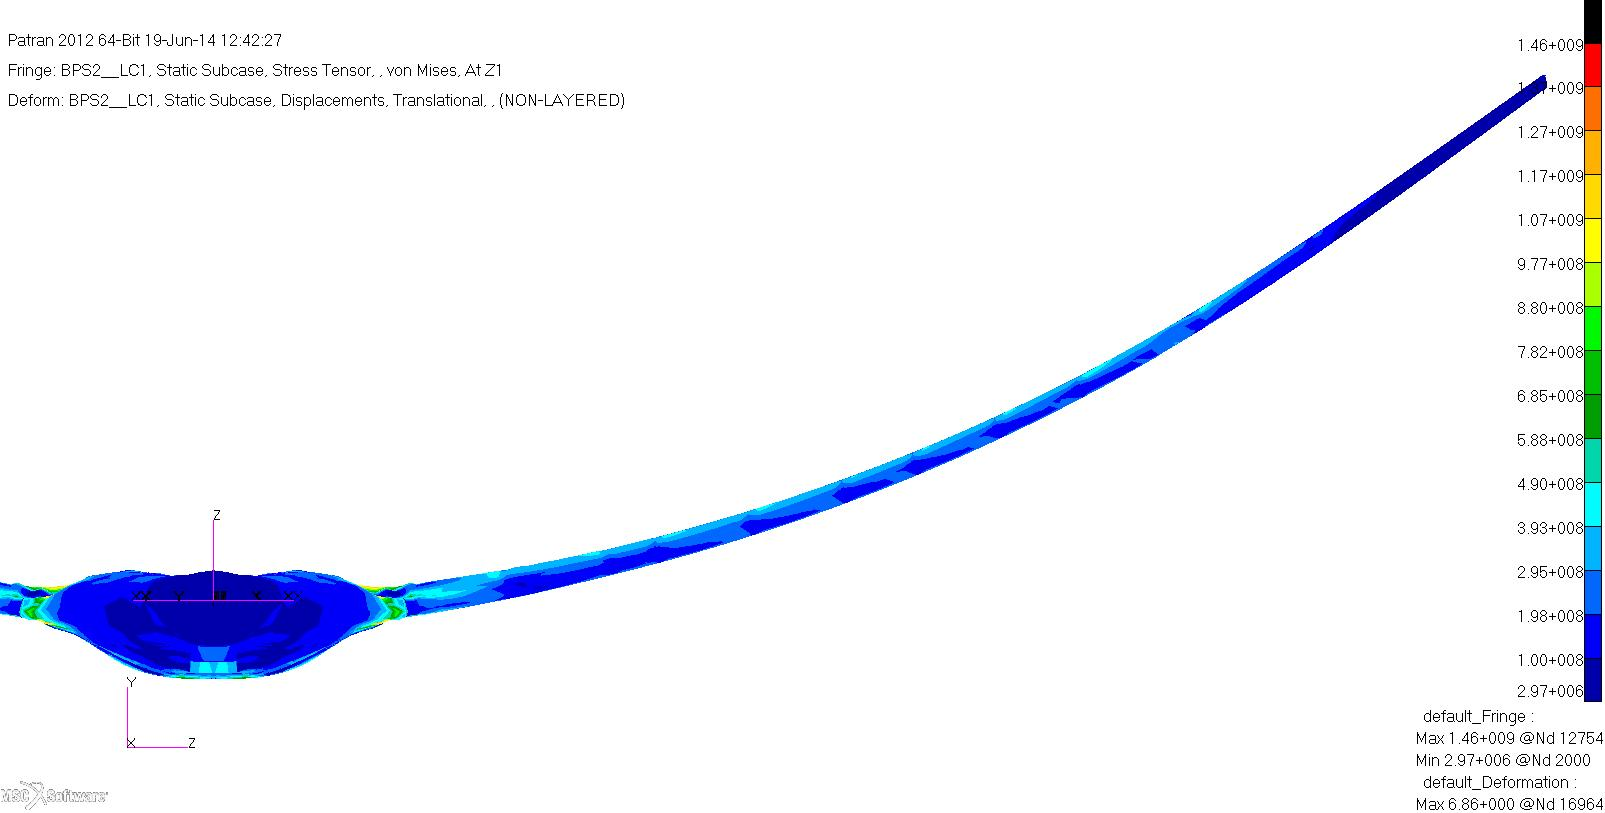
\includegraphics[width=0.8\textwidth]{patran/rear_deformed}
\caption{Вид сзади, деформированное состояние конструкции гипотетического БПЛА}
\label{fig:patranRearDeformed}
\end{figure}


%\begin{figure}[H]
%\centering
%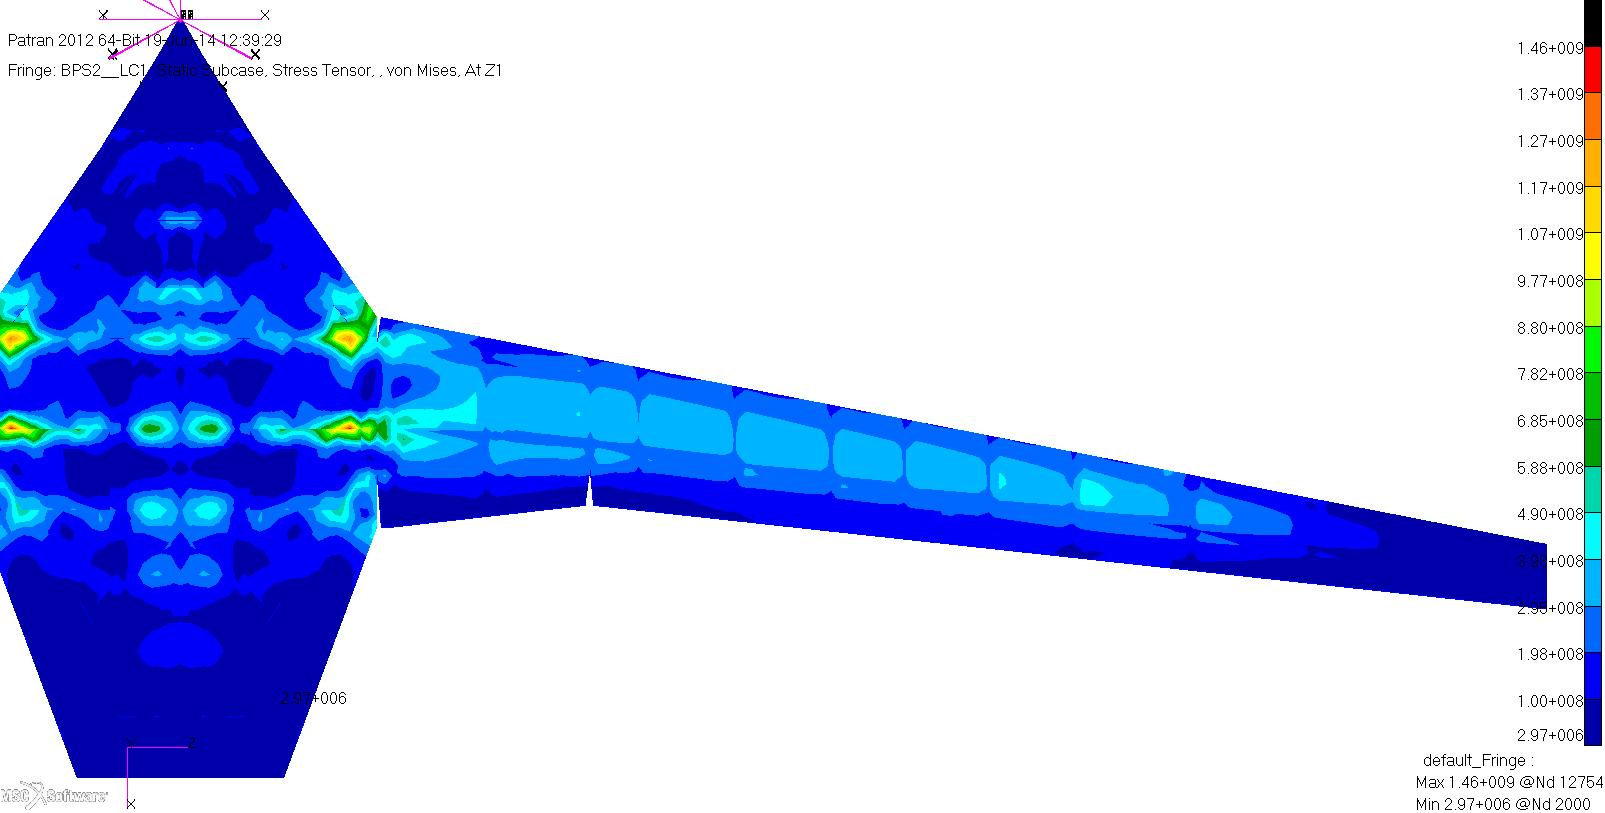
\includegraphics[width=0.7\textwidth]{patran/bottom}
%\caption{НДС конструкции гипотетического БПЛА. Вид снизу}
%\label{fig:patranBottom}
%\end{figure}
%
%
%\begin{figure}[H]
%\centering
%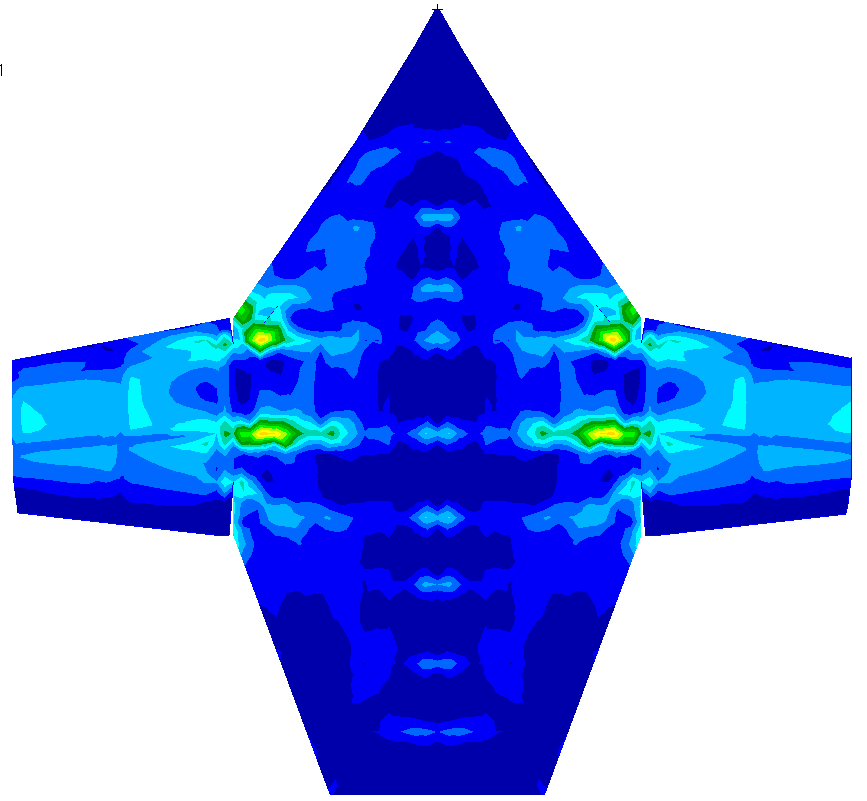
\includegraphics[width=0.7\textwidth]{patran/top}
%\caption{НДС конструкции гипотетического БПЛА. Вид сверху}
%\label{fig:patranTop}
%\end{figure}


\begin{figure}[H]
\centering
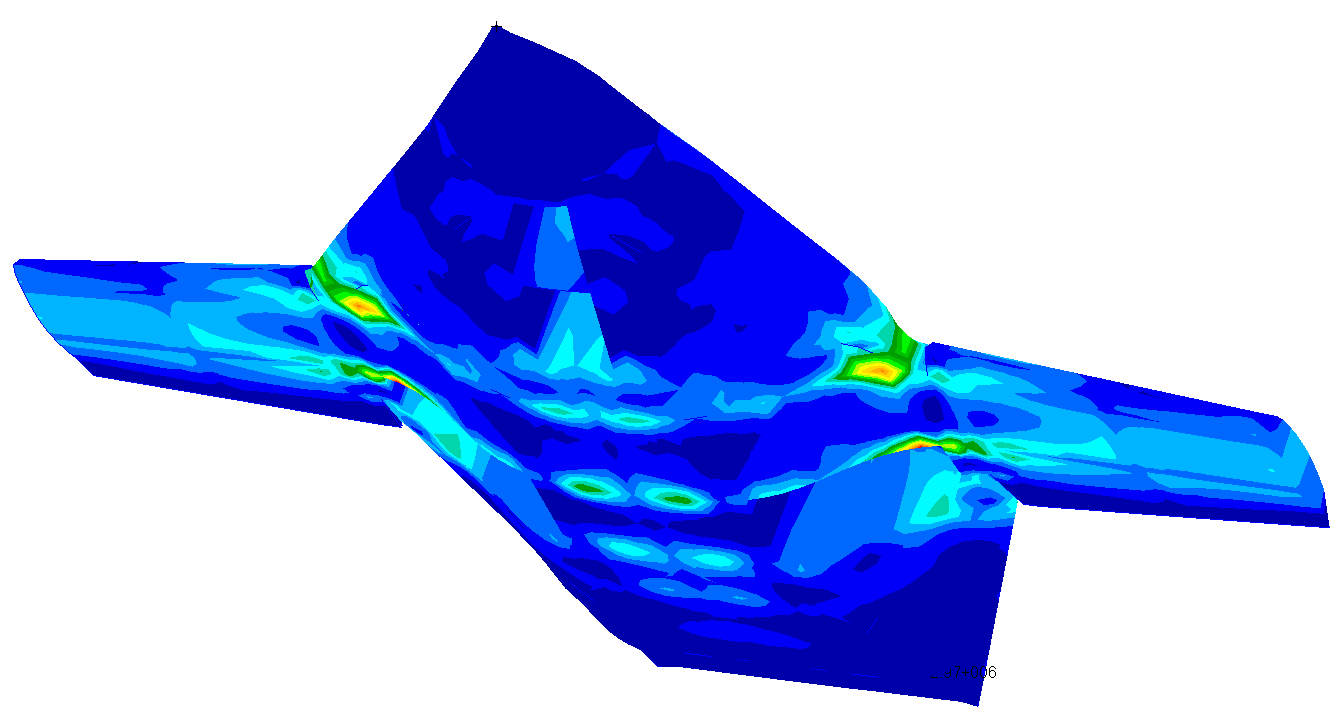
\includegraphics[width=0.8\textwidth]{patran/bottom_iso}
\caption{НДС конструкции гипотетического БПЛА. Вид в изометрии снизу}
\label{fig:patranBottomIso}
\end{figure}

\begin{figure}[H]
\centering
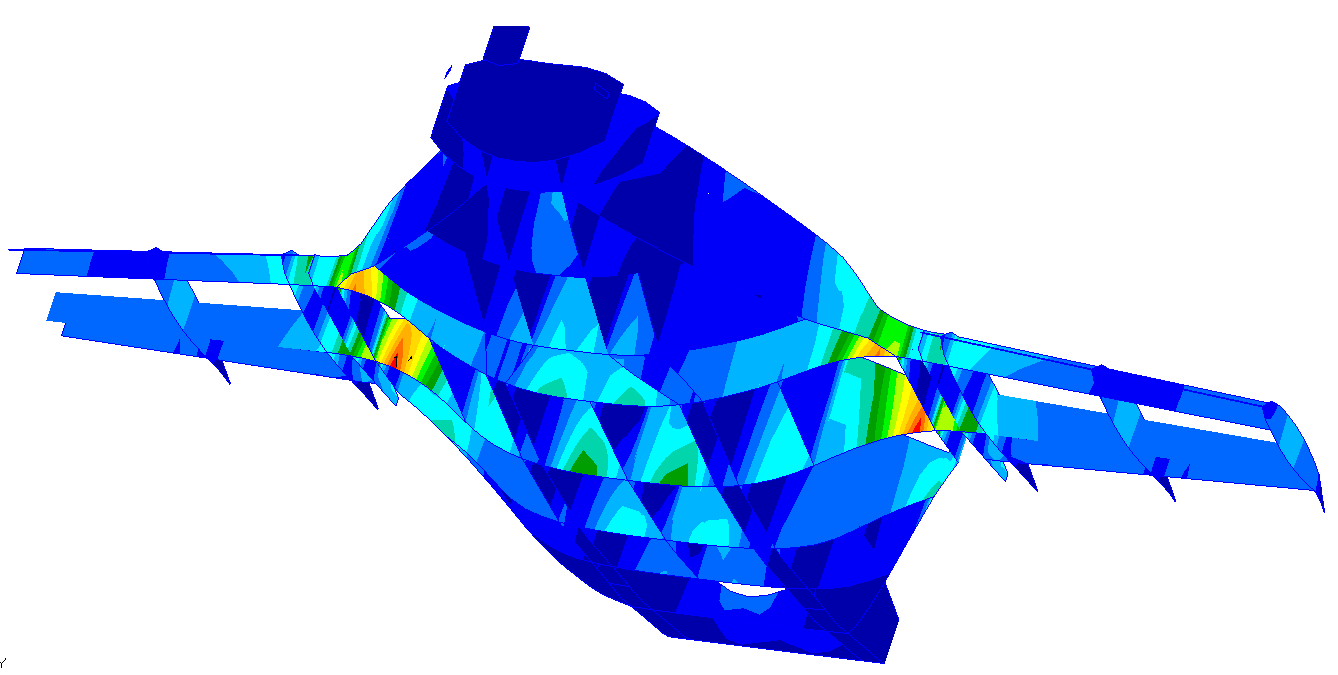
\includegraphics[width=0.8\textwidth]{patran/bottom_iso_noskin}
\caption{НДС конструкции гипотетического БПЛА. Вид снизу в изометрии без обшивки}
\label{fig:patranBottomIsoWithoutSkin}
\end{figure}

\begin{figure}[H]
\centering
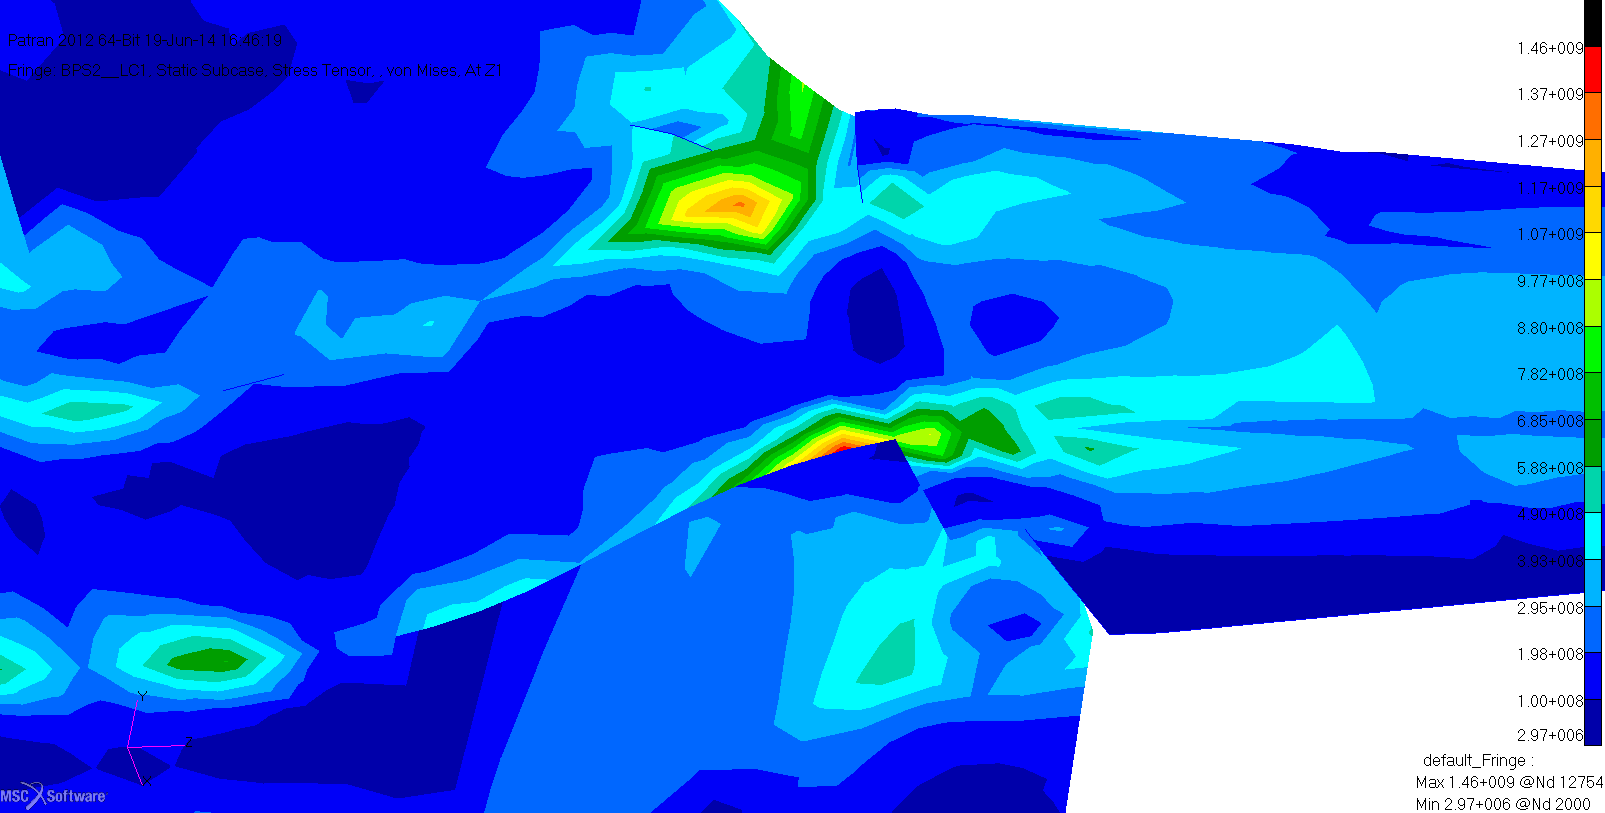
\includegraphics[width=0.8\textwidth]{patran/bottom_zoom}
\caption{НДС конструкции гипотетического БПЛА. Вид на стык крыла с фюзеляжем снизу в изометрии}
\label{fig:patranBottomIsoZoom}
\end{figure}


\begin{figure}[H]
\centering
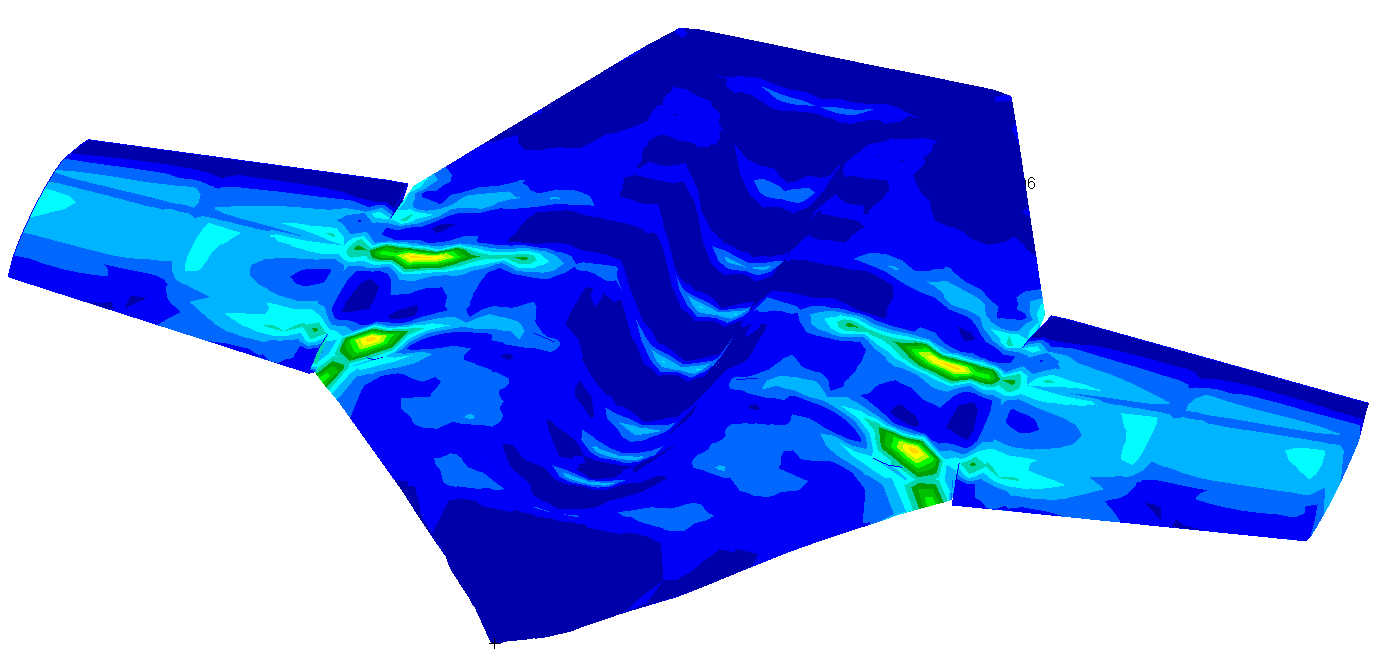
\includegraphics[width=0.8\textwidth]{patran/top_iso}
\caption{НДС конструкции гипотетического БПЛА. Вид сверху в изометрии}
\label{fig:patranTopIso}
\end{figure}

\begin{figure}[H]
\centering
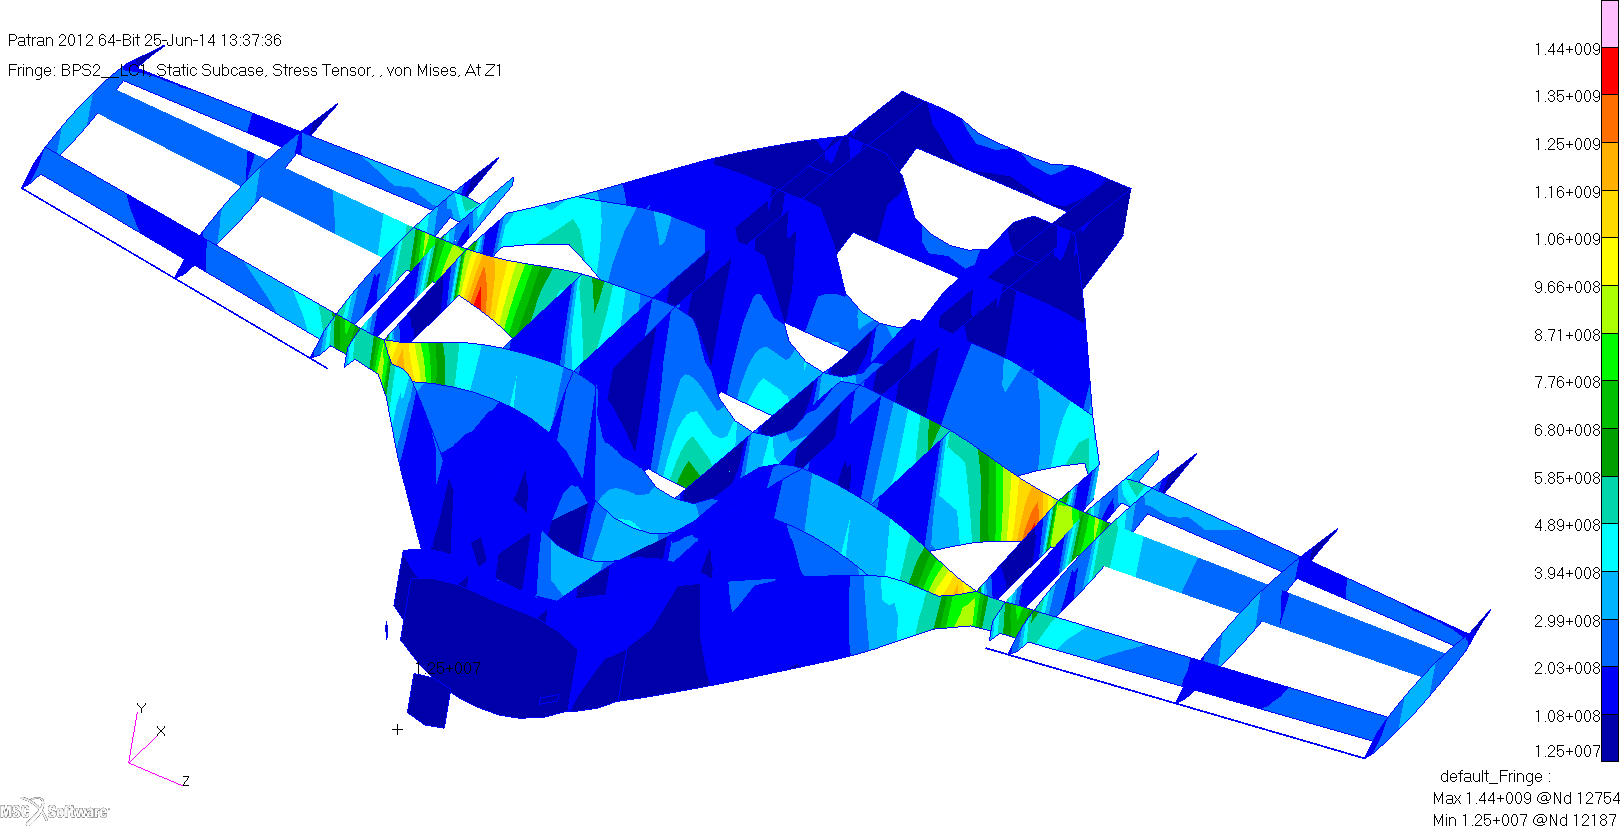
\includegraphics[width=0.8\textwidth]{patran/top_iso_noskin}
\caption{НДС конструкции гипотетического БПЛА. Вид сверху в изометрии без обшивки}
\label{fig:patranTopIsoWithoutSk}
\end{figure}
 \paragraph{Крепление хвостовой части к кессону центроплана} 
\label{sec:pants}
\begin{figure}[H]
\centering
\def\svgwidth{\textwidth}
\input{figures/IsoviewOfPants.pdf_tex}
%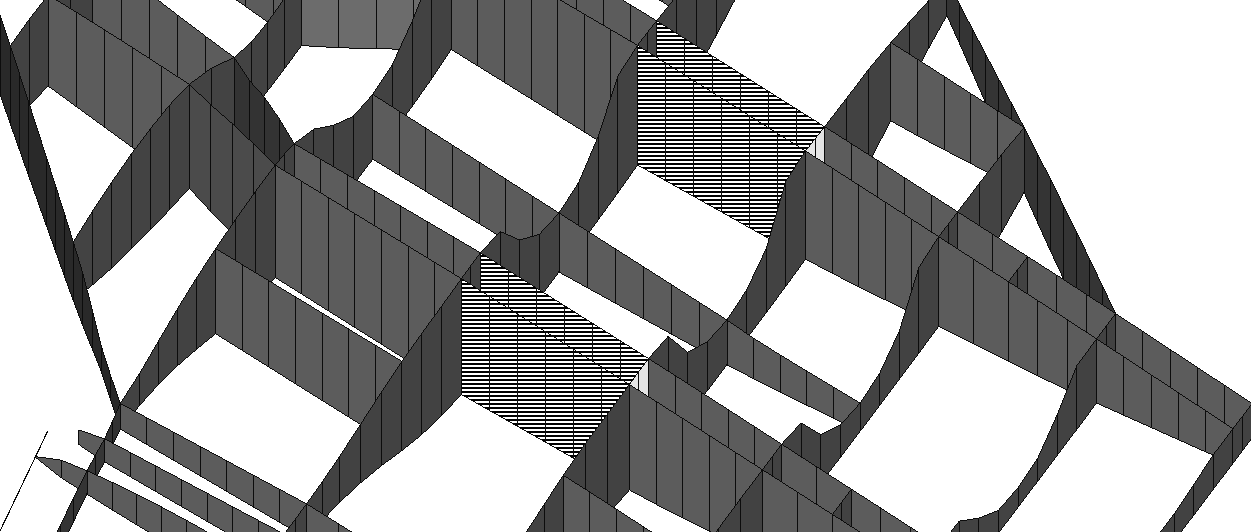
\includegraphics[width=0.6\textwidth]{IsoviewOfPantsBW}
\caption{Вид каркаса фюзеляжа}
\label{fig:IsoviewOfPants}
\end{figure}


Для частичной валидации решения, полученного в результате определния рациональных параметров (см. предыдущий раздел), была решена модельная задача по оценке устойчивости центральных стенок, обеспечивающих крепление хвостовой части гипотетического БПЛА к его центроплану (данные стенки обозначены на Рис.~\ref{fig:IsoviewOfPants} серой заливкой, светло-серой заливкой обозначены зоны основных узлов крепления двигателя). Эти стенки были нагружены перерезывающими усилиями, и необходима была проверка их по условиям устойчивости, которая не проводилась для этих элементов конструкции в процессе определения рациональных параметров. НДС стенок был оценен на основе аналитических формул. Схема нагружения модельных стенок показана на Рис.\ref{fig:IsoviewOfPantsModel}.

\begin{figure}[H]
\centering
%\def\svgwidth{0.9\textwidth}
\input{figures/IsoviewOfPantsModel.pdf_tex}
\caption{Схема нагружения модельных стенок}
\label{fig:IsoviewOfPantsModel}
\end{figure}

%
%\begin{figure}[H]
%\centering
%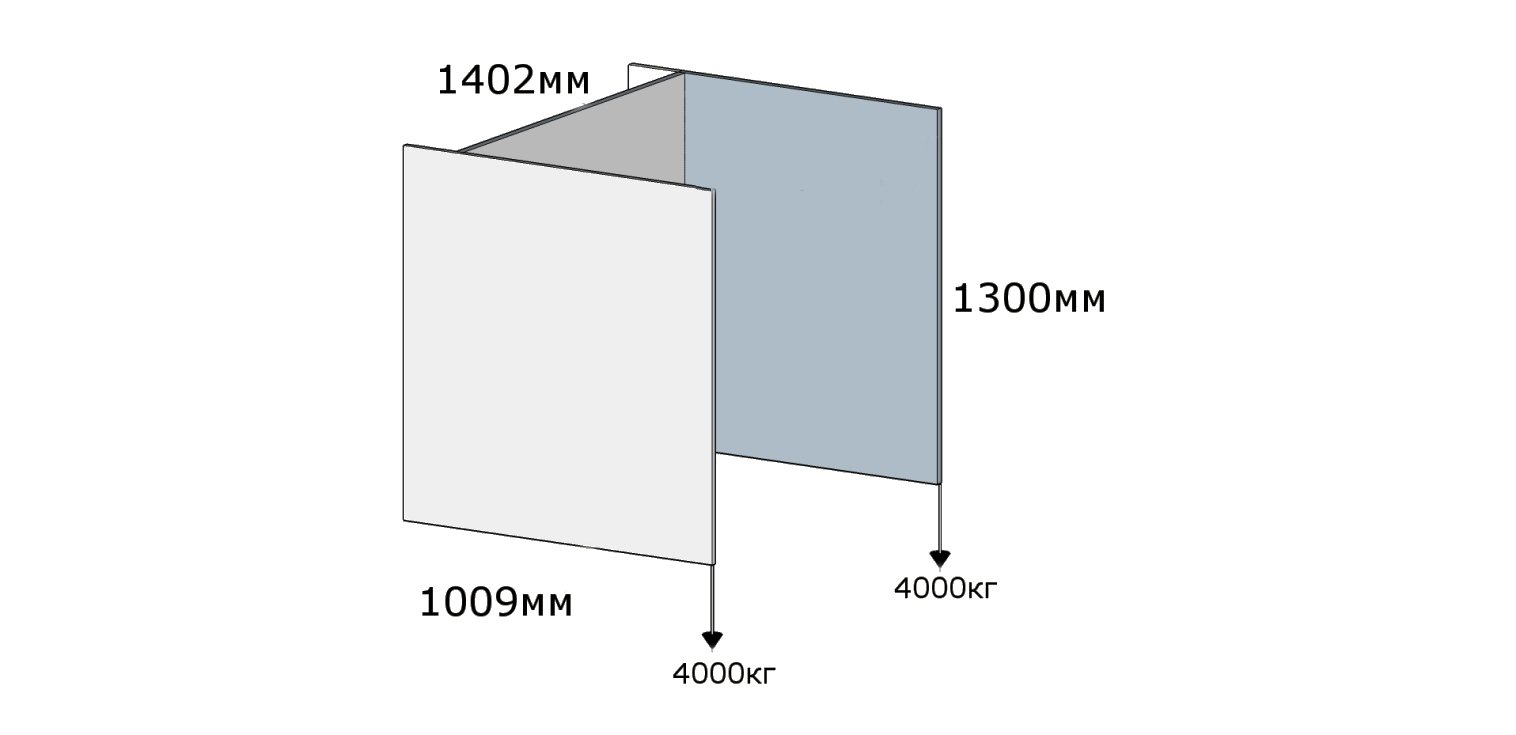
\includegraphics[width=0.8\textwidth]{IsoviewOfPantsModel}
%\caption{Схема нагружения модельных стенок}
%\label{IsoviewOfPantsModel}
%\end{figure}


Уровень нагружения был оценен по величинам касательных напряжений. Касательные напряжения в пластине при чистом сдвиге равны

\begin{equation}
\tau=\frac{3}{2}\cdot\frac{Q}{bh}
\end{equation}
Критические по устойчивости касательные напряжения в пластине при чистом сдвиге равны \cite{Volmir}:

\begin{equation}
\tau_\text{кр}=\frac{K}{12}\frac{\pi^2D}{b^2h} = \frac{K}{12}\frac{\pi^2E}{(1-\mu^2)}\left(\frac{h}{b}\right)^2,\, K=5.34 + 4\frac{a}{b},
\end{equation}
где $a$ - размер пластины вдоль направления действия силы, $b$ - размер пластины поперек направления действия силы, $h$ - толщина пластины, $D$ - изгибная жесткость пластины, $E$ - модуль Юнга, $\mu$ - модуль Пуассона материала пластины, $Q$ - приложенная сила.
Допускаемые толщины найдем из условия:

\begin{equation}
\tau_\text{кр} \geq \tau  
\end{equation}

\begin{equation}
h \geq \sqrt[3]{\frac{3\cdot12}{2}\frac{Qb\cdot(1-\mu^2)}{k\pi^2E}}
\end{equation}

Подставляя значения, получим:

\begin{equation}
Q=\frac{8000}{n}\text{кгс},\,a=1300\text{мм},\,b=1009\text{мм},\,\mu=0.3,\,E=7000\frac{\text{кгс}}{\text{мм}^2}
\end{equation}

\begin{equation}
h \geq \sqrt[3]{\frac{18\cdot8000\cdot1000\cdot(1-\mu^2)}{k\pi^2En}} = \frac{5.67}{\sqrt[3]{n}} 
\end{equation}

Таким образом, для случаев $n = 2$ и $n = 4$  были получены минимальные допустимые толщины, 
равные:

\begin{equation}
h\geq4.50\text{мм},\,n=2
\end{equation}
\begin{equation}
h\geq2.83\text{мм},\,n=4
\label{eq:pants_n4}
\end{equation}

Рациональные значения толщин исследуемых обшивок, полученные в данном проектировочном исследовании, оказались меньше ($h = 1\text{мм}$), чем приведенные в \ref{eq:pants_n4}. Таким образом, выполнение условий по устойчивости этих стенок привело к увеличению их толщин. Более рациональным способом увеличения сдвиговой жесткости этих стенок является использование ферменных подкрепляющих элементов.
%\subsubsection{Фюзеляжная часть центроплана}

Другим проблемным местом была фюзеляжная часть центроплана. Из-за требований компоновки, а именно интеграции двигателя, центроплан необходимо делать изогнутым (Рис.\ref{fig:centroplan}). Это вносит дополнительные трудности в виде увеличения веса по сравнению с прямым центропланом. Исследованию фюзеляжной части центроплана (выделена серым на Рис.\ref{fig:centroplan}) посвящена глава \ref{chap:SolvingModel}.

\begin{figure}[ht]
\centering
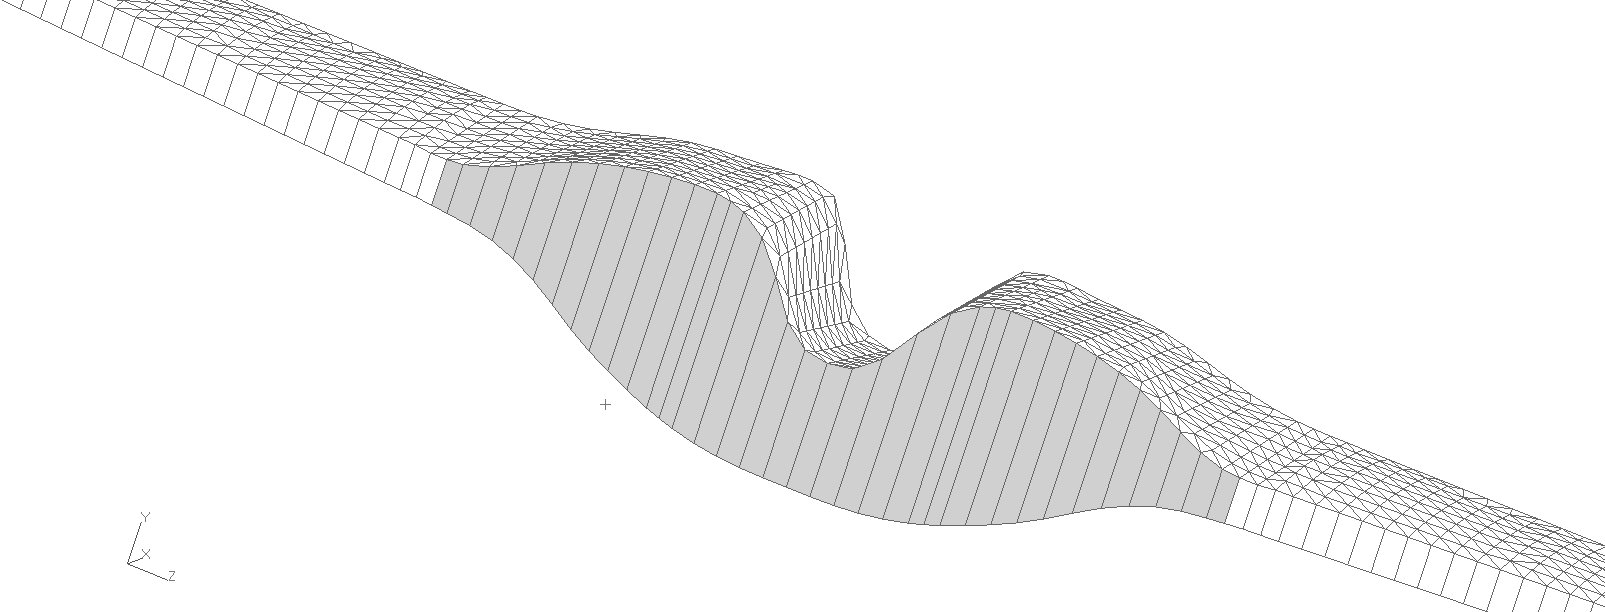
\includegraphics[width=0.6\textwidth]{centroplan}
\caption{Изогнутый центроплан с выделением исследуемой части}
\label{fig:centroplan}
\end{figure}
